\documentclass[10pt,a4paper]{article}
\usepackage[margin=1.8cm]{geometry}
\usepackage[T1]{fontenc}
\usepackage{lmodern}
\usepackage{booktabs,tabularx,array}
\usepackage{enumitem}
\usepackage[table]{xcolor}
\usepackage{hyperref}
\usepackage{titlesec}
\usepackage{microtype}
\usepackage{pgfplots}
\usepackage{listings}
\pgfplotsset{compat=1.17}

\setlist{nosep,leftmargin=1.2em}
\titlespacing*{\section}{0pt}{8pt}{3pt}
\titlespacing*{\subsection}{0pt}{6pt}{2pt}
\titleformat{\section}{\large\bfseries}{\thesection}{0.6em}{}
\titleformat{\subsection}{\normalsize\bfseries}{\thesubsection}{0.6em}{}
\setlength{\parskip}{3pt}
\setlength{\parindent}{0pt}
\setlength{\emergencystretch}{2em}
\hypersetup{colorlinks=true,urlcolor=blue,linkcolor=black}
\newcommand{\cf}{ContractForge}
\newcommand{\code}[1]{\texttt{\small #1}}

\definecolor{okgreen}{HTML}{2E7D32}
\definecolor{weakamber}{HTML}{C17A00}
\definecolor{failred}{HTML}{B42318}
\definecolor{rowgray}{HTML}{F2F4F7}

\lstset{basicstyle=\ttfamily\footnotesize,backgroundcolor=\color{rowgray},frame=none,
        columns=fullflexible,keepspaces=true,xleftmargin=4pt,xrightmargin=4pt,aboveskip=4pt,belowskip=4pt}

% one issue = what happens / evidence / why it matters / proposed fix
\newcommand{\what}{\par\smallskip\textbf{What happens.}~}
\newcommand{\evidence}{\par\smallskip\textbf{Evidence.}~}
\newcommand{\why}{\par\smallskip\textbf{Why it matters.}~}
\newcommand{\fix}{\par\smallskip\textbf{Proposed fix.}~}

\title{\vspace{-1.3cm}\textbf{\cf: Results of chain-v4 on the PURE Dataset}\\[2pt]
\large L0 $\rightarrow$ L1 $\rightarrow$ L2 on 18 SRS documents, and the issues they show}
\author{Bavya Sri Kilari (2025701029), Akshith K (2024111004), Vivek R (2019112020)\\
\small Autonomous Software Engineering, Monsoon 2026, IIIT Hyderabad}
\date{\small 13 November 2026 \quad Repository: \href{https://github.com/Ohshit-ak/AUTOSE-Leaniers}{\nolinkurl{github.com/Ohshit-ak/AUTOSE-Leaniers}}}

\begin{document}
\maketitle
\vspace{-0.9cm}

% =====================================================================
\section{Summary}
We ran the full pipeline on all 18 SRS documents in \code{Requirements/}: the 16 new PURE documents plus gamma~j and video search.
Every run finished. Out of \textbf{484} specs that entered L1/L2, \textbf{344 (71\%)} were verified end to end in the
strict setting and \textbf{366 (76\%)} with fallback. These headline numbers look good, but they overstate what the pipeline
achieves. The main problems are:
\begin{itemize}
\item \textbf{Almost half of the specs are weak.} 227 of 484 specs (47\%) can be satisfied by code that only copies input
      fields and returns constants. Counting only non-trivial specs, \textbf{150 (31\%)} are verified end to end (Issue~1).
\item \textbf{Decomposition is almost never exercised.} 435 of 484 specs (90\%) are routed as single-step. Only 11.3
      two-component architectures were accepted per repetition, and only \textbf{5} chains (1\%) verified end to end (Issue~2).
\item \textbf{L2 failures are almost all PO3.} The model writes a function that does not establish the contract's \code{post};
      usually it just copies the input (Issue~3).
\item \textbf{The parser keeps only 9\% of SRS items}, and almost nothing from two documents (get real: 1 of 110,
      peering: 1 of 228). The main cause is the rule that a requirement needs a modal verb (Issue~4).
\item \textbf{L0 loses 214 of the 698 parsed requirements} before L1, and the end-to-end rate does not count them (Issue~5).
\item \textbf{Specs are not checked against the requirement text.} A verified spec can contain conditions the requirement
      never states (Issue~6).
\item \textbf{The repetitions show little spread, and L0 ran only once}, so the ranges understate run-to-run variance (Issue~7).
\end{itemize}

\subsection{Run setup}
\begin{tabularx}{\linewidth}{@{}lX@{}}
\toprule
Documents   & 18 SRS XML files (16 new PURE documents + gamma~j + video search) \\
Model       & \code{qwen2.5-7b-instruct} (Q4\_K\_M, llama.cpp), temperature 0.2 (0.7 on restart); open-weight only \\
Harness     & chain-v4, commit \code{1b2599c}, clean tree in every run (\code{git\_dirty: false}) \\
Jobs        & Slurm 75464--75468, five jobs in parallel (\code{runs/qwen-pure-all.sbatch}), GTX 1080 Ti \\
Repetitions & L0: one run (seed 42). L1+L2: three repetitions (seeds 42, 43, 44) in two settings, strict and fallback \\
Numbers     & Mean over the three repetitions. Per-document details: \code{runs/<doc>/qwen-chain-v4/summary.md} \\
\bottomrule
\end{tabularx}

\subsection{Terms used in this report}
\begin{tabularx}{\linewidth}{@{}lX@{}}
\toprule
L0 & The model turns one requirement into a Lean spec (\code{Input}, \code{Output}, \code{pre}, \code{post}). The harness checks
     that it compiles and accepts a good example; the L0.5 review then accepts it or sends it back. \\
L1 & Architecture. If \code{post} has an intermediate result, the model splits the spec into two contracts
     $A : \mathit{Input} \to \mathit{Mid}$ and $B : \mathit{Mid} \to \mathit{Output}$. Otherwise the spec is \emph{single}:
     its one component is the spec itself, with no model call. \\
L2 & The model writes one Lean function per component; the harness proves PO3 for each. \\
PO1 / PO2 / PO3 & PO1: $A$'s guarantee gives $B$'s assumption. PO2: $A$ then $B$ refines the spec. PO3: the function meets its contract. \\
end to end & Lean accepts one file with the spec, the architecture, PO1--PO3 and \code{theorem system\_ok : Spec.Satisfies \dots}. \\
strict / fallback & Strict: a spec that needs a split fails if the split fails. Fallback: it is then implemented as one
     component (\emph{single-fallback}). \\
weak spec & A spec that an implementation made only of copied input fields and constants satisfies. Verified code for it may be a stub. \\
non-trivial e2e & End to end on a spec that is not weak, so the verified code had to compute something. \\
\bottomrule
\end{tabularx}

% =====================================================================
\section{Where the requirements go}
Totals over all 18 documents. The L1/L2 rows are means of three repetitions (strict setting).

\begin{center}
\begin{tabular}{@{}lrr@{}}
\toprule
Stage & count & \% of chain input \\
\midrule
Items in the SRS XML files                     & 7{,}849 & \\
Kept by the parser                             & 698     & \\
L0 spec compiles in Lean                       & 607     & \\
L0 spec checked (accepts a good example)       & 541     & \\
Accepted by the L0.5 review (chain input)      & 484     & 100\% \\
\midrule
Verified end to end, strict                    & 344     & 71\% \\
\quad \dots{} of which on a non-trivial spec   & 150     & 31\% \\
\quad \dots{} of which a real two-component chain & 5    & 1\% \\
\bottomrule
\end{tabular}
\end{center}

The parser removes about 91\% of the XML items. Most of those are prose, headings and non-normative sections, which is
intended, but see Issue~4. L0 loses another 214 of the 698 parsed items before L1. The biggest drop after that is the gap
between ``verified'' (344) and ``verified on a non-trivial spec'' (150).

% =====================================================================
\section{Results per document}
Figure~\ref{fig:perdoc} splits each document's specs into three parts: verified on a non-trivial spec (green), verified but
on a weak spec where a stub would also pass (amber), and not verified (red). Table~\ref{tab:perdoc} gives the numbers.

\begin{figure}[h]
\centering
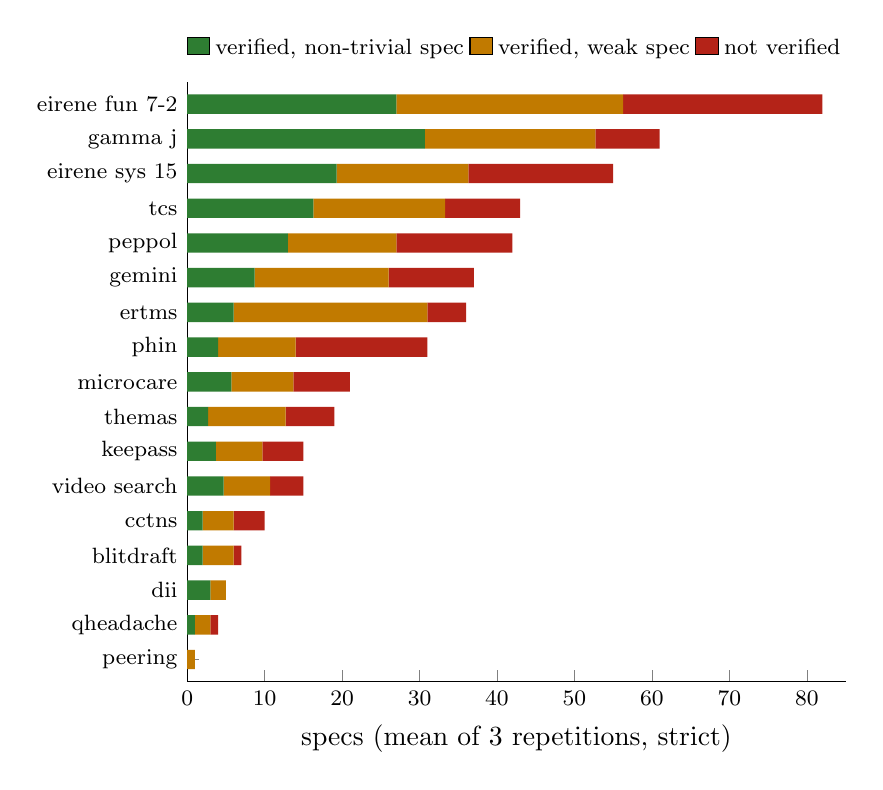
\begin{tikzpicture}
\begin{axis}[
  xbar stacked, width=0.82\linewidth, height=9.2cm, bar width=7pt,
  xmin=0, xmax=85, xlabel={specs (mean of 3 repetitions, strict)},
  symbolic y coords={peering,qheadache,dii,blitdraft,cctns,video search,keepass,themas,microcare,phin,ertms,gemini,peppol,tcs,eirene sys 15,gamma j,eirene fun 7-2},
  ytick=data, y tick label style={font=\footnotesize}, x tick label style={font=\footnotesize},
  legend style={at={(0.5,1.02)},anchor=south,legend columns=3,font=\footnotesize,draw=none},
  enlarge y limits=0.04, axis x line*=bottom, axis y line*=left,
]
\addplot[fill=okgreen,draw=none] coordinates {
  (27,eirene fun 7-2) (30.7,gamma j) (19.3,eirene sys 15) (16.3,tcs) (13,peppol) (8.7,gemini) (6,ertms) (4,phin)
  (5.7,microcare) (2.7,themas) (3.7,keepass) (4.7,video search) (2,cctns) (2,blitdraft) (3,dii) (1,qheadache) (0,peering)};
\addplot[fill=weakamber,draw=none] coordinates {
  (29.3,eirene fun 7-2) (22,gamma j) (17,eirene sys 15) (17,tcs) (14,peppol) (17.3,gemini) (25,ertms) (10,phin)
  (8,microcare) (10,themas) (6,keepass) (6,video search) (4,cctns) (4,blitdraft) (2,dii) (2,qheadache) (1,peering)};
\addplot[fill=failred,draw=none] coordinates {
  (25.7,eirene fun 7-2) (8.3,gamma j) (18.7,eirene sys 15) (9.7,tcs) (15,peppol) (11,gemini) (5,ertms) (17,phin)
  (7.3,microcare) (6.3,themas) (5.3,keepass) (4.3,video search) (4,cctns) (1,blitdraft) (0,dii) (1,qheadache) (0,peering)};
\legend{verified{,} non-trivial spec, verified{,} weak spec, not verified}
\end{axis}
\end{tikzpicture}
\caption{End-to-end outcome per document (strict). get real 0.2 is not shown: it has no chain specs.}
\label{fig:perdoc}
\end{figure}

\begin{table}[h]
\centering\small
\setlength{\tabcolsep}{4pt}
\rowcolors{2}{white}{rowgray}
\begin{tabular}{@{}lrrrrrllrlr@{}}
\toprule
Document & XML & parsed & specs & single & 2-comp & e2e strict & e2e fallb. & weak & non-triv.\ e2e & min \\
\midrule
0000 - cctns           & 151  & 22  & 10 & 9  & 0   & 6 (60\%)     & 6 (60\%)     & 4  & 2 (20\%)    & 3.4 \\
0000 - gamma j         & 274  & 54  & 61 & 57 & 1   & 52.7 (86\%)  & 54 (89\%)    & 24 & 30.7 (50\%) & 11.9 \\
1995 - gemini          & 1012 & 54  & 37 & 33 & 1.3 & 26 (70\%)    & 28 (76\%)    & 21 & 8.7 (23\%)  & 7.5 \\
1998 - themas          & 234  & 30  & 19 & 16 & 0.3 & 12.7 (67\%)  & 14.7 (77\%)  & 11 & 2.7 (14\%)  & 5.2 \\
1999 - dii             & 213  & 8   & 5  & 5  & 0   & 5 (100\%)    & 5 (100\%)    & 2  & 3 (60\%)    & 0.5 \\
1999 - tcs             & 453  & 70  & 43 & 39 & 0   & 33.3 (78\%)  & 35 (81\%)    & 20 & 16.3 (38\%) & 11.5 \\
2003 - qheadache       & 163  & 4   & 4  & 4  & 0   & 3 (75\%)     & 3 (75\%)     & 2  & 1 (25\%)    & 1.3 \\
2005 - microcare       & 440  & 34  & 21 & 19 & 0   & 13.7 (65\%)  & 16 (76\%)    & 10 & 5.7 (27\%)  & 5.2 \\
2005 - phin            & 196  & 43  & 31 & 28 & 0   & 14 (45\%)    & 15 (48\%)    & 13 & 4 (13\%)    & 10.5 \\
2006 - eirene sys 15   & 1258 & 79  & 55 & 45 & 3   & 36.3 (66\%)  & 41.7 (76\%)  & 22 & 19.3 (35\%) & 15.1 \\
2007 - get real 0.2    & 110  & 1   & 0  & 0  & 0   & --           & --           & 0  & --          & 0 \\
2007 - eirene\_fun\_7-2 & 656 & 126 & 82 & 72 & 1.7 & 56.3 (69\%)  & 61 (74\%)    & 35 & 27 (33\%)   & 22.8 \\
2007 - ertms           & 208  & 51  & 36 & 36 & 0   & 31 (86\%)    & 31 (86\%)    & 27 & 6 (17\%)    & 4.6 \\
2008 - keepass         & 408  & 28  & 15 & 12 & 1.3 & 9.7 (64\%)   & 10.7 (71\%)  & 9  & 3.7 (24\%)  & 4.4 \\
2008 - peering         & 228  & 1   & 1  & 1  & 0   & 1 (100\%)    & 1 (100\%)    & 1  & 0 (0\%)     & 0.1 \\
2009 - peppol approved & 1665 & 59  & 42 & 41 & 0   & 27 (64\%)    & 27.3 (65\%)  & 16 & 13 (31\%)   & 10.6 \\
2009 - video search    & 112  & 21  & 15 & 11 & 2.7 & 10.7 (71\%)  & 10.7 (71\%)  & 6  & 4.7 (31\%)  & 5.0 \\
2010 - blitdraft       & 68   & 13  & 7  & 7  & 0   & 6 (86\%)     & 6 (86\%)     & 4  & 2 (29\%)    & 1.1 \\
\midrule
\rowcolor{white}
\textbf{Total} & \textbf{7849} & \textbf{698} & \textbf{484} & \textbf{435} & \textbf{11.3} & \textbf{344 (71\%)} &
  \textbf{366 (76\%)} & \textbf{227} & \textbf{150 (31\%)} & \textbf{121} \\
\bottomrule
\end{tabular}
\caption{Per-document results. \emph{XML}: items in the SRS. \emph{specs}: L0 specs accepted into L1/L2. \emph{single}:
routed without a split. \emph{2-comp}: two-component architectures accepted by L1 (strict). \emph{min}: minutes per
repetition (strict and fallback averaged). Fractional values are means over three repetitions. gamma~j and video search reuse
their frozen L0 run (\code{qwen-v10.1/rep1}), made from an earlier parse, so their \emph{parsed} and \emph{specs} columns are
not directly comparable.}
\label{tab:perdoc}
\end{table}

% =====================================================================
\clearpage
\section{Issues, explained}
The issues are ordered by how much they change how the results should be read. Each one gives what happens, the evidence
from these runs, why it matters, and a proposed fix. None of the fixes have been made yet.

% ---------------------------------------------------------------------
\subsection*{Issue 1. Weak specs inflate the headline numbers}
\what An L0 spec is \emph{weak} when a function that only copies input fields and returns constants satisfies it. The harness
already flags these (\code{spec\_check.trivial}) but still lets them through. Their ``verified code'' can be a stub, so a large
part of the end-to-end count is not evidence that the model wrote working code.

\evidence
\begin{center}
\begin{tabular}{@{}lrr@{}}
\toprule
 & count & share of chain specs \\
\midrule
chain specs                              & 484 & 100\% \\
weak specs                               & 227 & 47\% \\
end to end (strict)                      & 344 & 71\% \\
end to end, non-trivial spec (strict)    & 150 & 31\% \\
end to end, non-trivial spec (fallback)  & 157 & 33\% \\
\bottomrule
\end{tabular}
\end{center}
The worst case is ertms: its headline is 86\% (31 of 36), but 27 of its 36 specs are weak and only 6 non-trivial specs
verify. phin has 14 specs end to end, of which only 4 are non-trivial.

\why The headline end-to-end rate (71\%) is more than twice the rate that shows real verified computation (31\%). If the report
leads with 71\%, a reviewer who opens a few verified files will find stubs.

\fix
\begin{itemize}
\item Report \textbf{non-trivial end to end} as the main metric everywhere (README, \code{results.md}, slides).
\item Send weak specs back to L0 with the trivial witness as feedback (``this constant implementation passes your spec, so the
      spec says too little''). This is the same loop L0 already uses for \code{rejects\_bad\_example}.
\end{itemize}

% ---------------------------------------------------------------------
\subsection*{Issue 2. Decomposition, the point of L1, is almost never tested}
\what L1 splits a spec into two components only if its \code{post} relates two output fields (an intermediate result). On these
documents almost every spec is routed as \emph{single}: the architecture is the spec itself and PO2 is
\code{Refines Spec Spec}, which is trivial.

\evidence
\begin{center}
\begin{tabular}{@{}lr@{}}
\toprule
 & mean per repetition (all documents) \\
\midrule
specs routed single (no split, no L1 model call)         & 435 of 484 (90\%) \\
specs that needed a split                                 & 49 \\
two-component architecture accepted (strict)              & 11.3 \\
two-component chain verified end to end                   & 5 \\
split failed, implemented as one component (fallback)     & 37 \\
\bottomrule
\end{tabular}
\end{center}
Why splits fail (L1 failure classes, strict, summed over documents): identity 21.3, po2 10.3, visibility 2.7,
unknown-field 2.0, type-error 1.3. \emph{Identity} means the model's first component only copies or restates its input,
so it does no real work. \emph{po2} means the two contracts compose, but together they do not imply the spec.
13 of the 18 documents have no chain verified end to end.

\why The project claims compositional verification (PO1 $\rightarrow$ PO2 $\rightarrow$ \code{system\_sound}), but on real
SRS documents that path runs for about 1\% of specs. The headline numbers are therefore results for one-component
verification and should not be presented as evidence for decomposition.

\fix
\begin{itemize}
\item Report the chain path separately (5 verified chains in total) and say clearly that the rest is single-step.
\item Check whether the routing rule is too strict: many specs have several independent output conditions that could be
      split but are not.
\item For identity failures, tell the model which field it must compute in \code{Mid}, the same way visibility errors
      already name the field to add.
\end{itemize}

% ---------------------------------------------------------------------
\subsection*{Issue 3. L2 failures are almost all PO3 (the code does not meet its contract)}
\what In L2 the model writes a Lean function and the harness tries to prove PO3. When a spec fails at L2, the reason is almost
always PO3, not a Lean syntax or type error. The model usually returns the input unchanged, or computes a simpler condition
than the one in \code{post}.

\evidence L2 component failure classes, summed over documents (mean per repetition): \textbf{po3 95.0}, unknown-field 3.7,
unknown-name 3.0, type-error 2.3, syntax 0.7. With fallback: po3 109.0.

phin is the clearest case. It has the lowest end-to-end rate (45\%). About 14 of its 28 single specs (13.7 on average) fail
PO3, the same ones in every repetition, even after 5 attempts. Its specs contain long $\leftrightarrow$ conditions over lists
of records. Example:
\begin{lstlisting}
-- phin 2.2.4.3a/S1, failed PO3 after 5 attempts
def SpecImpl (x : Input) : Output :=
  { valid := x.exposures.Nodup,
    exposures := x.exposures }
-- PO3: these parts of Spec.post are not established:
--   o.valid = true <-> o.exposures.length = i.exposures.length /\
--     forall e in i.exposures, ... e.level != "" /\ e.type in ["intimate", ...] /\
--     0 < e.time /\ 0 < e.frequency /\ 0 < e.proximity
\end{lstlisting}

\why This is where the model's coding ability limits the pipeline. Retrying with the same feedback does not help: specs that
fail do so in all three repetitions, after 5 attempts each.

\fix
\begin{itemize}
\item Give the model the failing conjunct as a short checklist (``\code{valid} must be true exactly when all of: \dots''),
      not only the Lean goal.
\item Measure how many failing specs are realizable at all: some \code{post}s may need input guarantees that \code{pre} does
      not give. The README already defines an \emph{unrealizable} class for this.
\end{itemize}

% ---------------------------------------------------------------------
\subsection*{Issue 4. The parser keeps too little from some documents}
\what The parser keeps a sentence as a requirement only if it has a normative modal verb (shall/must/will/should/can) and
something to formalise. The modal rule is the largest single filter, and it fails on documents that are written without
modals or that mark requirements with \code{<req>} tags instead.

\evidence
\begin{center}
\begin{tabular}{@{}lr@{}}
\toprule
Drop reason (all 18 documents) & items \\
\midrule
no normative modal (shall/must/will/should/can)                  & 3{,}521 \\
no state change, data relation or quantity to formalise          & 1{,}985 \\
non-normative section (purpose, references, user classes, \dots) & 871 \\
vague wording                                                    & 431 \\
UI only / UI steps                                               & 204 \\
overview or scope section, platform choice, SLA, other           & 136 \\
\bottomrule
\end{tabular}
\end{center}
\textbf{get real 0.2} keeps 1 of 110 items. The document contains no ``shall'' or ``must'' at all; it is a website description
written as prose. Its one spec was flagged in L0.5, so the chain step ran on 0 specs, and the summary step exited with an
error because there was no \code{l1l2.json} to read.

\textbf{peering} keeps 1 of 228 items. Its authors marked 25 items explicitly as \code{<req>}, but wrote them as statements
(``The format for service information description is defined''), so the modal rule drops them.

\why The documents with the least ``shall'' language are the ones the pipeline cannot use at all. Results on PURE are
therefore biased toward documents written in the classic ``The system shall \dots'' style, and the report should say so.

\fix
\begin{itemize}
\item Let elements the author explicitly tagged \code{<req>} skip the modal check. They would still go through the other
      filters. This is a general rule, not specific to one document.
\item Report the parser yield per document (it ranges from 0.4\% to 25\%) so readers can see this bias.
\item Make the summary step write an empty summary instead of exiting with an error when there are 0 specs.
\end{itemize}

% ---------------------------------------------------------------------
\subsection*{Issue 5. L0 loses about a third of the parsed requirements}
\what Between the parser and L1, a requirement must compile as a Lean spec, pass the harness checks, and be accepted by the
L0.5 review. Each step removes some of them.

\evidence
\begin{center}
\begin{tabular}{@{}lrr@{}}
\toprule
Stage (all 18 documents) & count & lost at this stage \\
\midrule
parsed requirements                       & 698 & \\
L0 spec compiles                          & 607 & 91 \\
L0 spec checked (accepts a good example)  & 541 & 66 \\
accepted by the L0.5 review (chain input) & 484 & 57 \\
\bottomrule
\end{tabular}
\end{center}
For example, phin has 43 parsed requirements: 37 compile, 34 pass the checks, and 31 are accepted (the review marked 8 as
\emph{redo} and 4 as \emph{review}). gamma~j and video search are not comparable, because their L0 run comes from an earlier parse.

\why These requirements never reach L1/L2. The end-to-end rate is measured against L0's accepted specs, not against the
requirements in the document, so it hides this loss.

\fix Report end-to-end rates against \emph{both} denominators: the specs accepted by L0, and the requirements kept by the
parser. Measured against the parser, strict non-trivial end to end is 150 of 698 (21\%).

% ---------------------------------------------------------------------
\subsection*{Issue 6. Specs are not checked against the requirement text (fidelity)}
\what End to end means the code satisfies the \emph{spec}. Nothing in the pipeline checks that the spec states what the
\emph{requirement} says. When a requirement is abstract, L0 makes up concrete conditions, and the result still counts as verified.

\evidence
\begin{lstlisting}
-- phin 2/I5, verified end to end
-- Requirement: "OM information must be exchangeable, based on established
--   standards, between systems involved in the investigation ... of a health event."
def SpecImpl (x : Input) : Output :=
  { exchanged := decide (x.omData.length <= 1024 /\ x.omData.toList.all Char.isAlphanum) }
\end{lstlisting}
The 1024-character limit and the alphanumeric rule do not appear in the requirement. This spec is verified, but what was
verified is not the requirement.

\why Without a fidelity measure, ``verified'' only means ``consistent with what the model decided the requirement means''.
Reviewers will ask about this first.

\fix
\begin{itemize}
\item Manually label a random sample of verified specs (for example 50) as faithful, partly faithful or invented, and report the rate.
\item Add a check that flags numbers and string constants in a spec that do not appear in the requirement text.
\end{itemize}

% ---------------------------------------------------------------------
\subsection*{Issue 7. The repetitions measure little variability, and L0 ran once}
\what L1 and L2 ran three times (seeds 42, 43, 44) on top of a \emph{single} L0 run. The three repetitions agree closely.

\evidence Of the 34 settings (17 documents with specs $\times$ strict/fallback), 17 give exactly the same end-to-end count in
all three repetitions. The rest differ by 1--4 specs (largest: gemini with fallback, 26--30 of 37). On ertms, 30 of the 36
specs got exactly the same L2 code in all three repetitions: most L2 calls succeed on the first attempt at temperature 0.2,
and the seed mostly matters on retries at temperature 0.7.

\why The small spread is real, but it only covers L1/L2. Which specs exist, how many are weak, and which are dropped are all
decided by L0, which ran once. So the error bars understate the true run-to-run variance.

\fix Run L0 with three seeds as well (at least on a few documents) and report the spread of the whole pipeline. Until then,
state that the current ranges cover L1/L2 only.

% =====================================================================
\section{Suggested order of work}
\begin{enumerate}
\item \textbf{Report honestly first (no new runs):} use non-trivial end to end as the main number, report the chain path
      separately, and give both denominators (Issues 1, 2, 5).
\item \textbf{Weak-spec feedback loop in L0} (Issue 1): the biggest effect on what the numbers mean.
\item \textbf{Fidelity sample} (Issue 6): a manual check of about 50 specs, needed before any claim about correctness.
\item \textbf{Parser: \code{<req>} skips the modal check, and the summary handles 0 specs} (Issue 4): small, general changes.
      Re-run only peering and get real.
\item \textbf{PO3 feedback and decomposition routing} (Issues 2, 3): larger research changes.
\end{enumerate}

\vfill
{\footnotesize Numbers from \code{runs/*/qwen-chain-v4*/summary.md}, \code{runs/*/qwen-v10.1/rep1/specs.json} and
\code{Requirements/parsed/*.json}.}

\end{document}
